Due to the subdivided structure of our agent, we had to entirely separate the training of our sub-agents.
For each agent, we defined a basic metric we wanted to measure its performance on, agreed on a method to calculate the
confidence to keep it as consistent as possible between all sub-agents, and decide on the best training method for all
of them.
For the actual training session, we used our private computers, as well as a Linux web server owned by Florian to allow
for longer runs without having to occupy our private devices for an extended period of time.

\subsection{Governor Training}
\label{subsec:training-governor}
As already mentioned in chapter~\ref{subsec:design-governor}, the governor was not using any \gls{ml} algorithms, but
rather consisted of static, handpicked parameters we determined by trial and error after all sub-agents had finished
their training.
We started out with equal weights, but soon realized that our agent is putting too much emphasis on survival, and the
survivor sub-agent was never allowing any other sub-agents to act - which did result in our agent surviving until the
end, but often losing after 400 turns due to the point tie-break.
% TODO: Insert results of adjusting bomber vs survivor weights.

\subsection{Survivor Training}
\subsubsection*{Florian}
\label{subsec:training-survivor}
For the survivor agent, we started out by deciding on an ideal localized survival strategy.
After some tests, our solution came out to be fairly similar to the one present in the rule-based agent provided by the
environment:
Our agent should avoid stepping into explosion tiles or the cross-shaped dangerous area surrounding any bomb, and if
caught inside of one, it should try to escape to the nearest free space, prioritizing turns around a corner over simply
moving away from the bomb.
There are some edge cases where this algorithm fails, for example, bombs reaching all the way into a dead end with no
free tiles to escape to - but because our agent was only supposed to have a localized vision, these cases would be outside
its vision range and thus not be detectable anyway.

As a target metric, we initially chose the number of survived turns, but soon discovered that the algorithm was not
converging very quickly.
After trying the number of survived bombs as a training metric and still not getting any satisfying results, we decided to
change our approach altogether:
Because our goal was to mimic an algorithm we already had, and not to find a solution to a problem we hadn't solved yet,
we didn't need to define a target metric.
Instead, we did exactly what we actually wanted our network to do:
Every time a move was requested by the environment, we ran our existing algorithm on the same input in parallel,
determined the \enquote{ideal move}, and stored this move as the target label for our weight adjustment later on.
This changed approach greatly improved the training runtime because we were now able to clearly label every single
move taken as \enquote{good} or \enquote{bad} in a vacuum, instead of having to analyze the entire game to determine the
quality of every move taken throughout it.

In addition, we were now able to replace our default training environment, the classic arena with three rule-based
agents, with a much smaller arena of 7x7 tiles (Excluding the border) and no agents, because the network simplifies
anything but bombs, free tiles, and explosions to solid tiles.
Another issue we noticed with our training was how the survivor agent barely had any reasons to act for move of the
time, which resulted in the network heavily favoring the \enquote{WAIT} action over anything else.
With the smaller environment and the missing agents, we had to somehow introduce a new source of bombs anyway, so
instead of agents placing bombs, we randomly placed bombs on free tiles, which allowed us to speed up training even more
and even solved the lethargy issue of our network.

\subsection{Bombing Training}
\subsubsection*{Keerthan Ugrani}
\label{subsec:training-bombing}

For the bombing agent, we understood the logical way of implementing the bomber agent and then converting it to features using a tensor, so that we could feed it to the model as the input for training purposes. In the training process, we calculate the total reward based on a set of predefined events that occurred during a game step. Each event type is associated with a specific reward value. We also provide a clear mapping logic between game events and their corresponding rewards, enabling the agent to learn from its interactions with the environment. We incentivize desirable behaviors (e.g., collecting coins, killing opponents) and penalize undesirable ones.

We also introduce a strategy for the agent to decide whether to choose actions based on the current knowledge (exploitation) or to explore new actions (exploration)

We keep checking on game events occurring and the end of each round. To handle the accumulation of experiences, train the network, update the network, and track game scores. These functions ensure that the agent learns from its interactions with the environment.

As a target metric, we initialized the highest rewards for killing the opponent and then exploding the crates. The agent when it reaches the dead-end corner and if either one is a crate then it places the bomb and earns the reward. Here we not only gave rewards for bombing up the opponent but also for collecting the coins placed randomly in the custom environment so that the agent learns to collect the coin after bombing up the crate. 

\begin{figure}
    \centering
    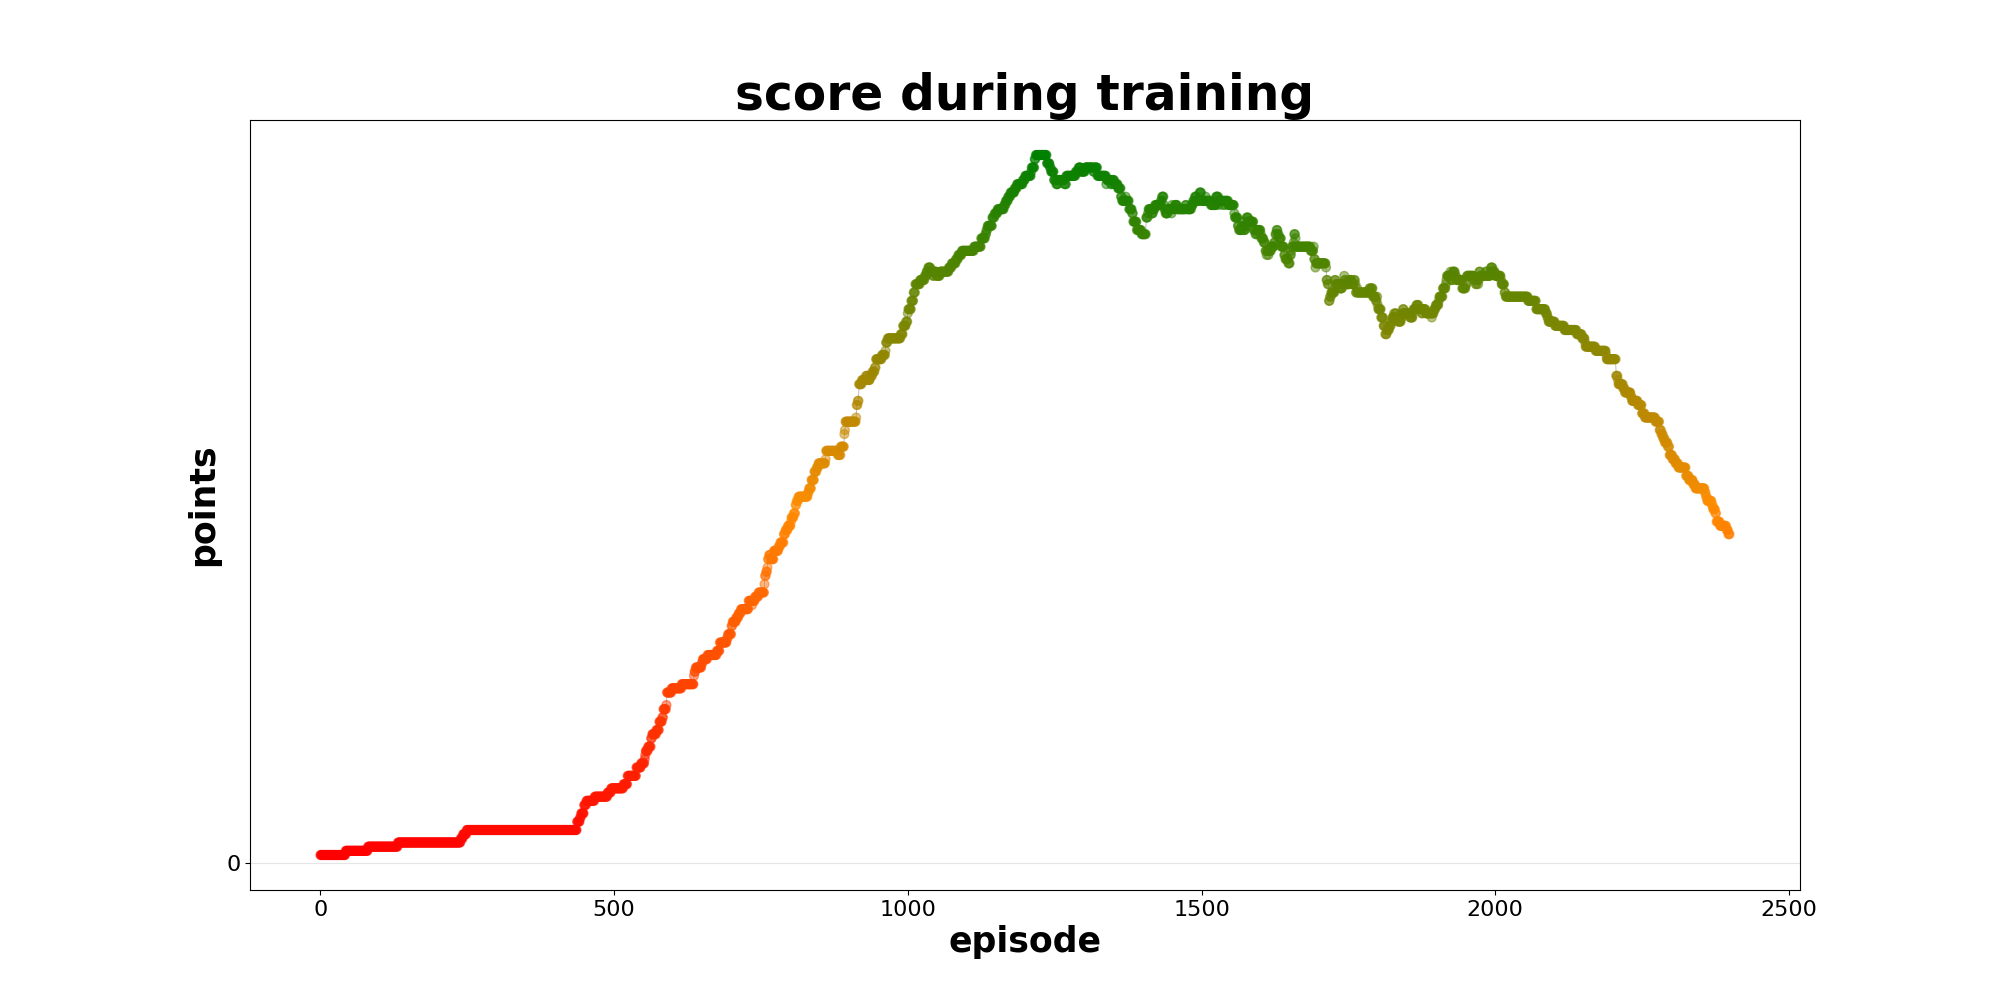
\includegraphics[width=0.5\textwidth]{src/training_progress.png}
    \caption{Training progress}
    \label{fig:enter-label}
\end{figure}
% TODO: Insert one subsection for every other agent here.
